In this chapter we present the results relevant to our discussed topics in the 
next chapter. To keep this chapter structured in a way that makes it easy to 
look up we divide our results into four main sections presenting model importance 
and feature importance for four cases:
\begin{enumerate}
    \item Models trained on CAMELS-GB \citep{CAMELS_GB}.
    \item Models trained on CAMELS \citep{CAMELS_US} in additiion to traditional 
        models provided by \citationneeded.
    \item Models trained on a dataset comprised of both CAMELS and CAMELS-GB.
    \item Models trained on CAMELS and validated on CAMELS-GB and vice-versa.
\end{enumerate}

\section{Models trained on CAMELS-GB}
In this sections we present the results related to model selection and feature 
importance when training and predicting on CAMELS-GB \citep{CAMELS_GB}. To act 
as a proof of concept of the feature importance method described in Chapter 
\ref{Feature selection} we also include the performance and feature importance of 
a model trained using dataset a (see Table \ref{attribute table}) in addition to
static attributes directly derived from the observed outcome.

\subsection{Performance}
\begin{figure}
    \centering
    \includegraphics{{results_section/camels_gb/cdf_val}.pdf}
    \caption{Cumulative distribution function of the NSE score of LSTM models trained 
    on CAMELS-GB \citep{CAMELS_GB}. "Overfit model" is a model deliberately trained 
    using static basin attributes derived from the runoff time series of the basins. 
    The other models are described in Table \ref{all models}.}
    \label{CAMELS-GB CDF validation}
\end{figure}

\subsection{Importance}
\section{Models trained CAMELS}
\subsection{Performance}
\begin{figure}
    \centering
    \includegraphics{{results_section/camels_us/cdf_val}.pdf}
    \caption{Cumulative distribution function of the NSE score of models trained 
    on CAMELS \citep{CAMELS_US}. "VIC" is the Variable Infiltration Capacity model 
    calibrated on CAMELS. "SAC-SMA" is the SACramento Soil Moisture Accounting 
    model calibrated on CAMELS. 
    These benchmarks are provided by \citet{CAMELS_hydroshare} and are originally 
    created by \citet{VICbench} and are trained per-basin as opposed to the other 
    models.
    The other models are described in Table \ref{all models} and are based on the 
    models originally trained by \citet{lstm_third_paper} but retrained for better 
    comparison with the other LSTM models in this thesis.}
    \label{CAMELS-US CDF validation}
\end{figure}
\subsection{Importance}
\section{Models trained on CAMELS and CAMELS-GB}
\subsection{Performance}
\begin{figure}
    \centering
    \includegraphics{{results_section/mixed/cdf_val}.pdf}
    \caption{Cumulative distribution function of the NSE score of LSTM models trained 
    on a dataset consisting of both CAMELS \citet{CAMELS_US} and CAMELS-GB \citep{CAMELS_GB}. 
    The models are described in Table \ref{all models}. The top figure shows the 
    performance of the models on CAMELS-GB and the bottom figure shows the performance 
    on CAMELS.}
    \label{mixed CDF validation}
\end{figure}
\subsection{Importance}
\section{Models trained for transfer learning between CAMELS and CAMELS-GB}
\subsection{Performance}
\begin{figure}
    \centering
    \includegraphics{{results_section/transfer/cdf_val}.pdf}
    \caption{Cumulative distribution function of the NSE score of LSTM models trained 
    on CAMELS \citep{CAMELS_US} and validated on a validation part of CAMELS as well as 
    the entirety of CAMELS-GB \citep{CAMELS_GB}. The top figure shows the 
    performance of the models on CAMELS-GB and the bottom figure shows the performance 
    on CAMELS.}
    \label{transfer CDF validation}
\end{figure}
\subsection{Importance}
\section{Test performance of best models}
Note that when doing model selection we do not look at test set performance, only 
performance on the cross validated train set.
%\begin{table}
%    \begin{adjustbox}{width=\textwidth}
%    \begin{tabular}{lr}
\toprule
{} &     Coeff \\
\midrule
Q95                   &  1.211018 \\
elev\_50               &  0.464968 \\
conductivity\_cosby\_50 &  0.443736 \\
intercept             &  0.443277 \\
porosity\_cosby\_50     &  0.409635 \\
conductivity\_hypres\_5 &  0.257509 \\
high\_prec\_dur         &  0.211253 \\
gauge\_easting         & -0.211231 \\
tawc                  & -0.326509 \\
elev\_max              & -0.349975 \\
conductivity\_cosby\_5  & -0.351292 \\
baseflow\_index\_ceh    & -0.417237 \\
bares\_perc            & -0.463398 \\
elev\_10               & -0.496951 \\
conductivity\_cosby\_95 & -0.839606 \\
porosity\_hypres\_5     & -1.030274 \\
low\_prec\_freq         & -1.055273 \\
dwood\_perc            & -1.288324 \\
p\_mean                & -2.015090 \\
ewood\_perc            & -2.146395 \\
urban\_perc            & -2.332153 \\
shrub\_perc            & -3.735298 \\
grass\_perc            & -4.010000 \\
crop\_perc             & -4.868455 \\
\bottomrule
\end{tabular}


%    \end{adjustbox}
%    \caption{Table for attempt at linear regression. This model is fit on the static
%    features as input values, and the NSE of an LSTM trained without static features
%    for each basin in the validation set. The $R^2$ score of this model is $\approx 0.5$}
%    \label{linreg_no_static_table}
%\end{table}
%In table \ref{linreg_no_static_table} we can see that our linear regression used to model 
%the relationship between NSE value of models and static features has decided that 
%several features are important. All these coefficients have a p-value $<0.5$. The 
%problem with this model was that it achieved an $R^2$ score of $\approx 0.5$, meaning 
%it does not actually explain the relationship well. We therefore choose to change 
%strategy for feature selection. 
\begin{comment}
\begin{figure}
    \includegraphics{{correlation_reduction/all_features/corr_and_dendrogram}.pdf}
    \caption{The Pearson correlation matrix and the corresponding hierarchial
    cluster of the training set before removing correlated features. The process
    of creating the dendrogram is described in chapter \ref{Feature selection}. 
    For readability's sake we cannot include every label in the correlation matrix.}
    \label{corr_matrix_full}
\end{figure}

\begin{figure}
    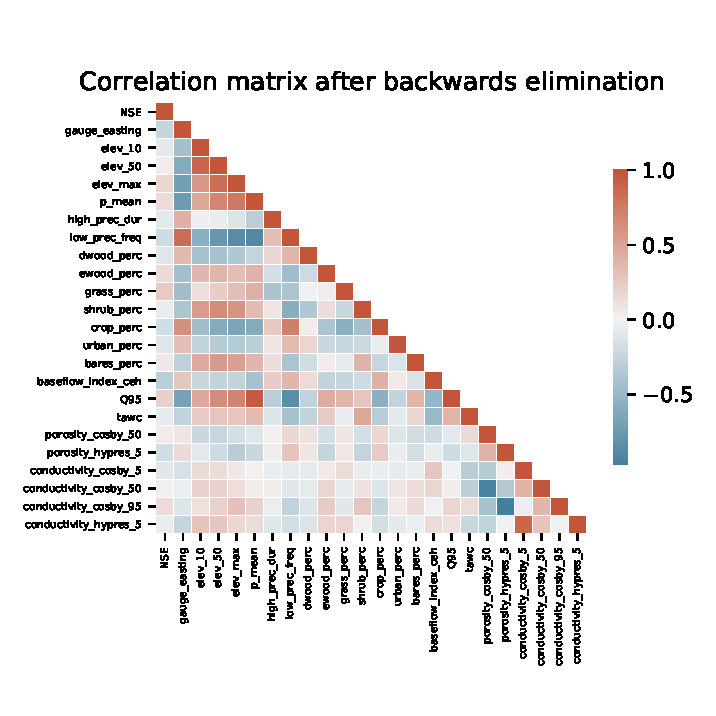
\includegraphics{reduced_matrix.pdf}
    \caption{Correlation matrix after backward selection}
    \label{corr_matrix_reduced}
\end{figure}

%\subsection{Performance of full model}
\begin{figure}
%\includegraphics[scale=1]{{permutation/all_features_cv/histogram_all}.pdf}
    \includegraphics{{figures/permutation/all_features_cv/histogram_all}.pdf}
\caption{The two most important (above) and least important (below) features according 
to the permutation test}
\label{Hist all}
\end{figure}



\begin{figure}
    \centering
    \includegraphics{{CDFs/mixed_model_comparisons}.pdf}
    \caption{top kjeks}
    \label{main cdf}
\end{figure}
\end{comment}
